\section{Theory}

\begin{figure}[htp]
    \centering
    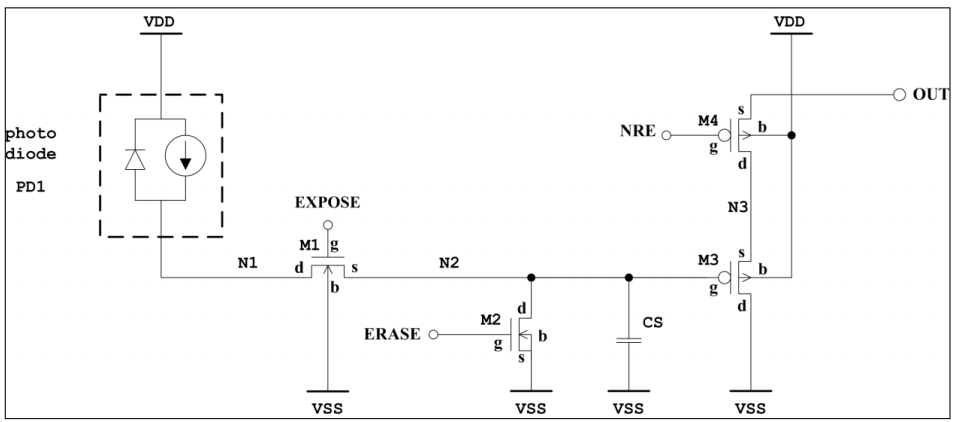
\includegraphics[scale=0.55]{Images/IC_Analog.PNG}
    \caption{Circuit diagram}
    \label{fig:AnalogC}
\end{figure} \\

Each pixel readout in the camera is shown in the figure \ref{fig:AnalogC}. 
The photo diode generates a current between 50pA and 750pA depending on the light conditions. Whenever a picture is taken the current is let through the M1 transistor and is used to charge the capacitor CS. The longer the transistor is open, the more current can flow into the capacitor. This allows to convert a current-driven signal into a voltage-driven signal.\\

The capacitor CS needs to scaled so it's possible to achieve the maximum dynamic range for the pixel with respect to the exposure time. The current stored in the capacitor needs to converge at the same time when the camera reaches maximum exposure time.       \\

The M3 transistor converts the voltage stored at CS into a differential resistance between N3 and VSS. The M4 transistor works as a switch, and the M1 transistor should be closed whenever a image is not being taken.





\newpage